\section{Figures}


\begin{figure}[htbp]
\centering
\begin{subfigure}[b]{.35 \textwidth}
	\centering
	\caption{}
	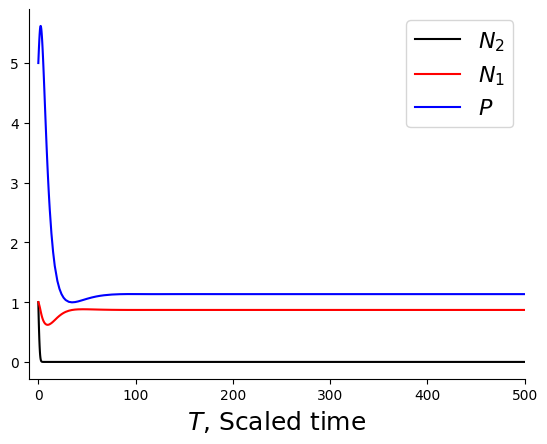
\includegraphics[width=\textwidth]{Figures/params_pop1_onex_1_plotall.png}
	\label{fig_onex_1}
\end{subfigure}
\begin{subfigure}[b]{.35 \textwidth}
	\centering
	\caption{}
	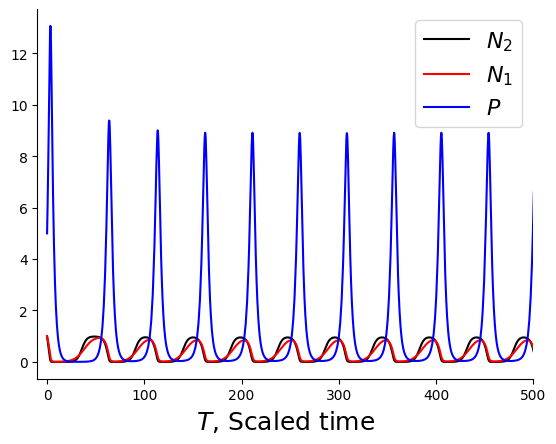
\includegraphics[width=\textwidth]{Figures/params_pop1_onex_2_plotall.png}
	\label{fig_onex_2}
\end{subfigure}
\begin{subfigure}[b]{.35 \textwidth}
	\centering
	\caption{}
	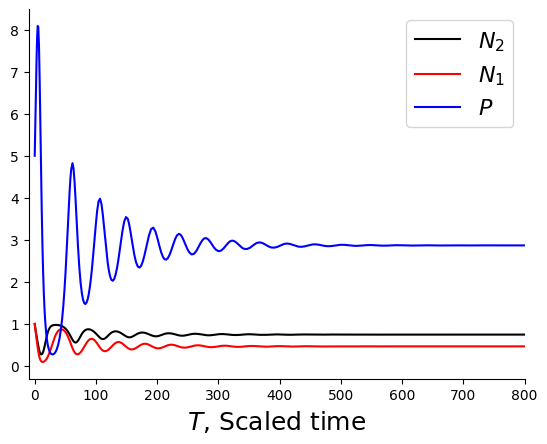
\includegraphics[width=\textwidth]{Figures/params_pop1_onex_4_plotall.png}
	\label{fig_onex_4}
\end{subfigure}
\begin{subfigure}[b]{.35 \textwidth}
	\centering
	\caption{}
	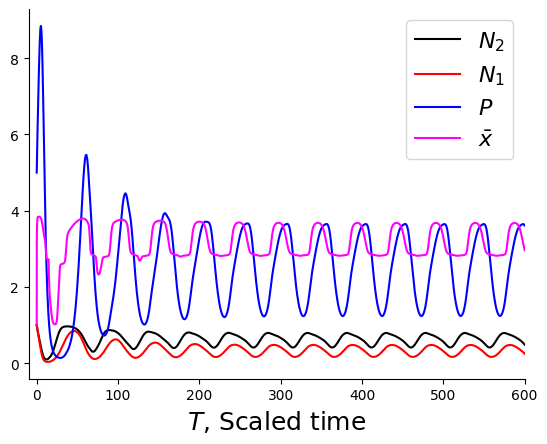
\includegraphics[width=\textwidth]{Figures/params_pop1_plotall.png}
	\label{fig_changex}
\end{subfigure}
\caption{A comparison of population dynamics  for all groups of the same size (panels (A) - (C)) and for a trajectory in which groups changing (panell (D)). For all panels, the parameters are $\xi = 2, \eta_1 = 0.2, \eta_2 = 0.4, A_1 = 0.5, \beta_1 = 10, \beta_2 = 1, H_1 = 2, H_2 = 2, \alpha_1(1) = 0.05, s_1 =2$, and $\alpha_2(x) = 0.95$ is constant, and the initial scaled population sizes are $P(0) =5, N_1(0) = N_2(0) = 1$. For panels (A) - (D), the scaled population sizes of predators, $P$, big prey, $N_1$, and small prey $N_2$, are shown in relation to scaled time, $T$, but in panel (D), the change in the expected group size that a randomly selected predator is part of, $\bar{x}$ is also shown versus time, $T$. For panels (A) - (C), the group size of predators if $x = 1, 2,$ and $4$ respectively. For the trajectory shown in panels $(D)$, the scaled group dynamics time constant is $T_x = 0.01$, and all predators are initially solitary.}
\label{compare_onegrp_fission_fusion}
\end{figure}